\documentclass[letterpaper,12pt]{article}
\usepackage[margin=14mm,top=18mm,bottom=17mm,headheight=14pt]{geometry}
\pdfmapfile{+cm.map}\pdfmapfile{+cmextra.map}
\usepackage{tikz,fancyhdr,amsmath,amssymb}
\usetikzlibrary{arrows.meta,patterns}
\pagestyle{fancy}\fancyhf{}\renewcommand{\headrulewidth}{0pt}
\fancyhead[L]{\small Week 49 / Four towers and differences / K--1}
\fancyfoot[L]{\small Bellingham Math Circle / Week 49 / F49-K-v3}
\fancyfoot[R]{\small\thepage}
\setlength{\parindent}{0pt}\setlength{\parskip}{0pt}
\begin{document}
\noindent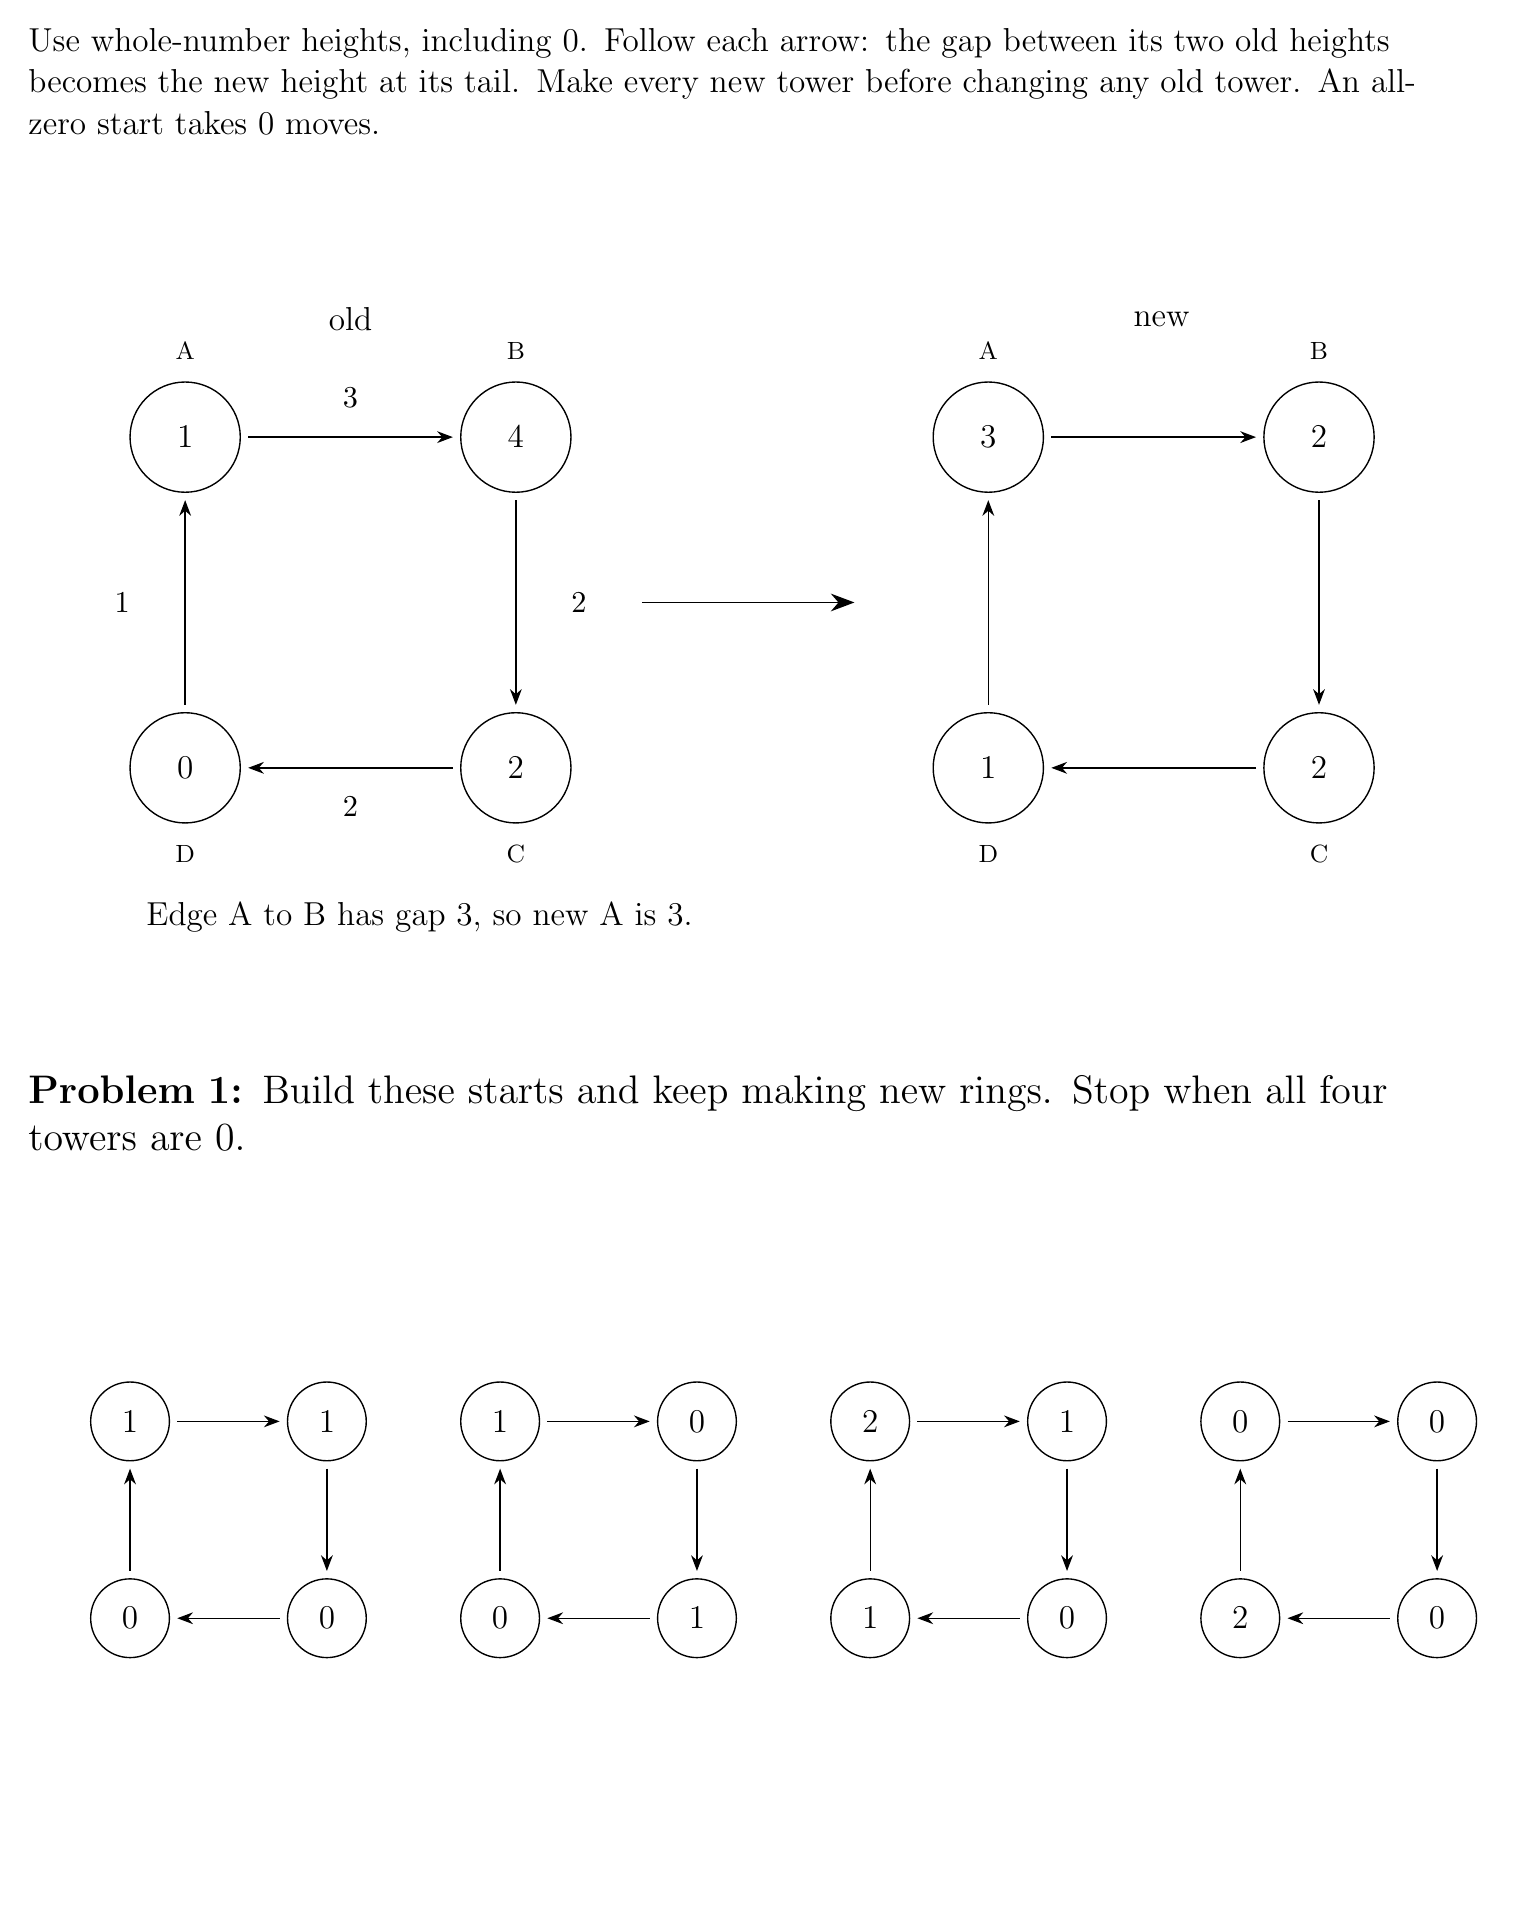
\begin{tikzpicture}[x=1mm,y=-1mm,line width=.5pt]
\path[use as bounding box] (0,0) rectangle (185,235);
\node[anchor=north west,inner sep=0pt,text width=180mm,font=\fontsize{12}{15}\selectfont] at (0,0) {Use whole-number heights, including 0. Follow each arrow: the gap between its two old heights becomes the new height at its tail. Make every new tower before changing any old tower. An all-zero start takes 0 moves.};
\node[anchor=center,inner sep=1pt,font=\fontsize{12}{14}\selectfont] at (41,37) {old};
\node[anchor=center,inner sep=1pt,font=\fontsize{12}{14}\selectfont] at (144,37) {new};
\draw[-{Stealth[length=2mm]}] (28.0,52.0) -- (54.0,52.0);
\node[anchor=center,inner sep=1pt,font=\fontsize{11}{13}\selectfont] at (41.0,47.0) {3};
\draw[-{Stealth[length=2mm]}] (62.0,60.0) -- (62.0,86.0);
\node[anchor=center,inner sep=1pt,font=\fontsize{11}{13}\selectfont] at (70.0,73.0) {2};
\draw[-{Stealth[length=2mm]}] (54.0,94.0) -- (28.0,94.0);
\node[anchor=center,inner sep=1pt,font=\fontsize{11}{13}\selectfont] at (41.0,99.0) {2};
\draw[-{Stealth[length=2mm]}] (20.0,86.0) -- (20.0,60.0);
\node[anchor=center,inner sep=1pt,font=\fontsize{11}{13}\selectfont] at (12.0,73.0) {1};
\draw[fill=white] (20,52) circle (7);
\node[anchor=center,inner sep=1pt,font=\fontsize{9}{11}\selectfont] at (20,41) {A};
\node[anchor=center,inner sep=1pt,font=\fontsize{13}{15}\selectfont] at (20,52) {1};
\draw[fill=white] (62,52) circle (7);
\node[anchor=center,inner sep=1pt,font=\fontsize{9}{11}\selectfont] at (62,41) {B};
\node[anchor=center,inner sep=1pt,font=\fontsize{13}{15}\selectfont] at (62,52) {4};
\draw[fill=white] (62,94) circle (7);
\node[anchor=center,inner sep=1pt,font=\fontsize{9}{11}\selectfont] at (62,105) {C};
\node[anchor=center,inner sep=1pt,font=\fontsize{13}{15}\selectfont] at (62,94) {2};
\draw[fill=white] (20,94) circle (7);
\node[anchor=center,inner sep=1pt,font=\fontsize{9}{11}\selectfont] at (20,105) {D};
\node[anchor=center,inner sep=1pt,font=\fontsize{13}{15}\selectfont] at (20,94) {0};
\draw[-{Stealth[length=3mm]}] (78,73) -- (105,73);
\draw[-{Stealth[length=2mm]}] (130.0,52.0) -- (156.0,52.0);
\draw[-{Stealth[length=2mm]}] (164.0,60.0) -- (164.0,86.0);
\draw[-{Stealth[length=2mm]}] (156.0,94.0) -- (130.0,94.0);
\draw[-{Stealth[length=2mm]}] (122.0,86.0) -- (122.0,60.0);
\draw[fill=white] (122,52) circle (7);
\node[anchor=center,inner sep=1pt,font=\fontsize{9}{11}\selectfont] at (122,41) {A};
\node[anchor=center,inner sep=1pt,font=\fontsize{13}{15}\selectfont] at (122,52) {3};
\draw[fill=white] (164,52) circle (7);
\node[anchor=center,inner sep=1pt,font=\fontsize{9}{11}\selectfont] at (164,41) {B};
\node[anchor=center,inner sep=1pt,font=\fontsize{13}{15}\selectfont] at (164,52) {2};
\draw[fill=white] (164,94) circle (7);
\node[anchor=center,inner sep=1pt,font=\fontsize{9}{11}\selectfont] at (164,105) {C};
\node[anchor=center,inner sep=1pt,font=\fontsize{13}{15}\selectfont] at (164,94) {2};
\draw[fill=white] (122,94) circle (7);
\node[anchor=center,inner sep=1pt,font=\fontsize{9}{11}\selectfont] at (122,105) {D};
\node[anchor=center,inner sep=1pt,font=\fontsize{13}{15}\selectfont] at (122,94) {1};
\node[anchor=north west,inner sep=0pt,text width=180mm,font=\fontsize{12}{15}\selectfont] at (15,111) {Edge A to B has gap 3, so new A is 3.};
\node[anchor=north west,inner sep=0pt,text width=180mm,font=\fontsize{14}{17}\selectfont] at (0,133) {\textbf{Problem 1:} Build these starts and keep making new rings. Stop when all four towers are 0.};
\draw[-{Stealth[length=2mm]}] (19.0,177.0) -- (32.0,177.0);
\draw[-{Stealth[length=2mm]}] (38.0,183.0) -- (38.0,196.0);
\draw[-{Stealth[length=2mm]}] (32.0,202.0) -- (19.0,202.0);
\draw[-{Stealth[length=2mm]}] (13.0,196.0) -- (13.0,183.0);
\draw[fill=white] (13,177) circle (5);
\node[anchor=center,inner sep=1pt,font=\fontsize{13}{15}\selectfont] at (13,177) {1};
\draw[fill=white] (38,177) circle (5);
\node[anchor=center,inner sep=1pt,font=\fontsize{13}{15}\selectfont] at (38,177) {1};
\draw[fill=white] (38,202) circle (5);
\node[anchor=center,inner sep=1pt,font=\fontsize{13}{15}\selectfont] at (38,202) {0};
\draw[fill=white] (13,202) circle (5);
\node[anchor=center,inner sep=1pt,font=\fontsize{13}{15}\selectfont] at (13,202) {0};
\draw[-{Stealth[length=2mm]}] (66.0,177.0) -- (79.0,177.0);
\draw[-{Stealth[length=2mm]}] (85.0,183.0) -- (85.0,196.0);
\draw[-{Stealth[length=2mm]}] (79.0,202.0) -- (66.0,202.0);
\draw[-{Stealth[length=2mm]}] (60.0,196.0) -- (60.0,183.0);
\draw[fill=white] (60,177) circle (5);
\node[anchor=center,inner sep=1pt,font=\fontsize{13}{15}\selectfont] at (60,177) {1};
\draw[fill=white] (85,177) circle (5);
\node[anchor=center,inner sep=1pt,font=\fontsize{13}{15}\selectfont] at (85,177) {0};
\draw[fill=white] (85,202) circle (5);
\node[anchor=center,inner sep=1pt,font=\fontsize{13}{15}\selectfont] at (85,202) {1};
\draw[fill=white] (60,202) circle (5);
\node[anchor=center,inner sep=1pt,font=\fontsize{13}{15}\selectfont] at (60,202) {0};
\draw[-{Stealth[length=2mm]}] (113.0,177.0) -- (126.0,177.0);
\draw[-{Stealth[length=2mm]}] (132.0,183.0) -- (132.0,196.0);
\draw[-{Stealth[length=2mm]}] (126.0,202.0) -- (113.0,202.0);
\draw[-{Stealth[length=2mm]}] (107.0,196.0) -- (107.0,183.0);
\draw[fill=white] (107,177) circle (5);
\node[anchor=center,inner sep=1pt,font=\fontsize{13}{15}\selectfont] at (107,177) {2};
\draw[fill=white] (132,177) circle (5);
\node[anchor=center,inner sep=1pt,font=\fontsize{13}{15}\selectfont] at (132,177) {1};
\draw[fill=white] (132,202) circle (5);
\node[anchor=center,inner sep=1pt,font=\fontsize{13}{15}\selectfont] at (132,202) {0};
\draw[fill=white] (107,202) circle (5);
\node[anchor=center,inner sep=1pt,font=\fontsize{13}{15}\selectfont] at (107,202) {1};
\draw[-{Stealth[length=2mm]}] (160.0,177.0) -- (173.0,177.0);
\draw[-{Stealth[length=2mm]}] (179.0,183.0) -- (179.0,196.0);
\draw[-{Stealth[length=2mm]}] (173.0,202.0) -- (160.0,202.0);
\draw[-{Stealth[length=2mm]}] (154.0,196.0) -- (154.0,183.0);
\draw[fill=white] (154,177) circle (5);
\node[anchor=center,inner sep=1pt,font=\fontsize{13}{15}\selectfont] at (154,177) {0};
\draw[fill=white] (179,177) circle (5);
\node[anchor=center,inner sep=1pt,font=\fontsize{13}{15}\selectfont] at (179,177) {0};
\draw[fill=white] (179,202) circle (5);
\node[anchor=center,inner sep=1pt,font=\fontsize{13}{15}\selectfont] at (179,202) {0};
\draw[fill=white] (154,202) circle (5);
\node[anchor=center,inner sep=1pt,font=\fontsize{13}{15}\selectfont] at (154,202) {2};
\end{tikzpicture}
\newpage
\noindent\begin{tikzpicture}[x=1mm,y=-1mm,line width=.5pt]
\path[use as bounding box] (0,0) rectangle (185,235);
\node[anchor=north west,inner sep=0pt,text width=180mm,font=\fontsize{14}{17}\selectfont] at (0,0) {\textbf{Problem 2:} Choose heights from 0 to 4. Find a start that lasts as many moves as you can; count the move that makes all four towers 0.};
\node[anchor=center,inner sep=1pt,font=\fontsize{12}{14}\selectfont] at (44,43) {old};
\node[anchor=center,inner sep=1pt,font=\fontsize{12}{14}\selectfont] at (141,43) {new};
\draw[-{Stealth[length=2mm]}] (37.0,71.0) -- (51.0,71.0);
\draw[-{Stealth[length=2mm]}] (70.0,90.0) -- (70.0,104.0);
\draw[-{Stealth[length=2mm]}] (51.0,123.0) -- (37.0,123.0);
\draw[-{Stealth[length=2mm]}] (18.0,104.0) -- (18.0,90.0);
\draw[fill=white,rounded corners=1mm] (0,53) rectangle ++(36,36);
\node[anchor=center,inner sep=1pt,font=\fontsize{9}{11}\selectfont] at (18,49) {A};
\draw[fill=white,rounded corners=1mm] (52,53) rectangle ++(36,36);
\node[anchor=center,inner sep=1pt,font=\fontsize{9}{11}\selectfont] at (70,49) {B};
\draw[fill=white,rounded corners=1mm] (52,105) rectangle ++(36,36);
\node[anchor=center,inner sep=1pt,font=\fontsize{9}{11}\selectfont] at (70,145) {C};
\draw[fill=white,rounded corners=1mm] (0,105) rectangle ++(36,36);
\node[anchor=center,inner sep=1pt,font=\fontsize{9}{11}\selectfont] at (18,145) {D};
\draw[-{Stealth[length=2mm]}] (134.0,71.0) -- (148.0,71.0);
\draw[-{Stealth[length=2mm]}] (167.0,90.0) -- (167.0,104.0);
\draw[-{Stealth[length=2mm]}] (148.0,123.0) -- (134.0,123.0);
\draw[-{Stealth[length=2mm]}] (115.0,104.0) -- (115.0,90.0);
\draw[fill=white,rounded corners=1mm] (97,53) rectangle ++(36,36);
\node[anchor=center,inner sep=1pt,font=\fontsize{9}{11}\selectfont] at (115,49) {A};
\draw[fill=white,rounded corners=1mm] (149,53) rectangle ++(36,36);
\node[anchor=center,inner sep=1pt,font=\fontsize{9}{11}\selectfont] at (167,49) {B};
\draw[fill=white,rounded corners=1mm] (149,105) rectangle ++(36,36);
\node[anchor=center,inner sep=1pt,font=\fontsize{9}{11}\selectfont] at (167,145) {C};
\draw[fill=white,rounded corners=1mm] (97,105) rectangle ++(36,36);
\node[anchor=center,inner sep=1pt,font=\fontsize{9}{11}\selectfont] at (115,145) {D};
\draw[-{Stealth[length=3mm]}] (78,97) -- (107,97);
\draw[] (20,176) rectangle ++(14,11);
\node[anchor=center,inner sep=1pt,font=\fontsize{12}{14}\selectfont] at (27,181.5) {};
\node[anchor=center,inner sep=1pt,font=\fontsize{9}{11}\selectfont] at (27,172) {A};
\draw[] (34,176) rectangle ++(14,11);
\node[anchor=center,inner sep=1pt,font=\fontsize{12}{14}\selectfont] at (41,181.5) {};
\node[anchor=center,inner sep=1pt,font=\fontsize{9}{11}\selectfont] at (41,172) {B};
\draw[] (48,176) rectangle ++(14,11);
\node[anchor=center,inner sep=1pt,font=\fontsize{12}{14}\selectfont] at (55,181.5) {};
\node[anchor=center,inner sep=1pt,font=\fontsize{9}{11}\selectfont] at (55,172) {C};
\draw[] (62,176) rectangle ++(14,11);
\node[anchor=center,inner sep=1pt,font=\fontsize{12}{14}\selectfont] at (69,181.5) {};
\node[anchor=center,inner sep=1pt,font=\fontsize{9}{11}\selectfont] at (69,172) {D};
\node[anchor=north west,inner sep=0pt,text width=85mm,font=\fontsize{12}{15}\selectfont] at (97,176) {Moves to zero: \rule{17mm}{.3pt}};
\draw[] (20,213) rectangle ++(14,11);
\node[anchor=center,inner sep=1pt,font=\fontsize{12}{14}\selectfont] at (27,218.5) {};
\node[anchor=center,inner sep=1pt,font=\fontsize{9}{11}\selectfont] at (27,209) {A};
\draw[] (34,213) rectangle ++(14,11);
\node[anchor=center,inner sep=1pt,font=\fontsize{12}{14}\selectfont] at (41,218.5) {};
\node[anchor=center,inner sep=1pt,font=\fontsize{9}{11}\selectfont] at (41,209) {B};
\draw[] (48,213) rectangle ++(14,11);
\node[anchor=center,inner sep=1pt,font=\fontsize{12}{14}\selectfont] at (55,218.5) {};
\node[anchor=center,inner sep=1pt,font=\fontsize{9}{11}\selectfont] at (55,209) {C};
\draw[] (62,213) rectangle ++(14,11);
\node[anchor=center,inner sep=1pt,font=\fontsize{12}{14}\selectfont] at (69,218.5) {};
\node[anchor=center,inner sep=1pt,font=\fontsize{9}{11}\selectfont] at (69,209) {D};
\node[anchor=north west,inner sep=0pt,text width=85mm,font=\fontsize{12}{15}\selectfont] at (97,213) {Moves to zero: \rule{17mm}{.3pt}};
\end{tikzpicture}
\newpage
\noindent\begin{tikzpicture}[x=1mm,y=-1mm,line width=.5pt]
\path[use as bounding box] (0,0) rectangle (185,235);
\node[anchor=north west,inner sep=0pt,text width=180mm,font=\fontsize{14}{17}\selectfont] at (0,0) {\textbf{Problem 3:} Find different starts that become all zeros in one move.};
\draw[-{Stealth[length=2mm]}] (29.0,47.0) -- (51.0,47.0);
\draw[-{Stealth[length=2mm]}] (60.0,56.0) -- (60.0,78.0);
\draw[-{Stealth[length=2mm]}] (51.0,87.0) -- (29.0,87.0);
\draw[-{Stealth[length=2mm]}] (20.0,78.0) -- (20.0,56.0);
\draw[fill=white] (20,47) circle (8);
\node[anchor=center,inner sep=1pt,font=\fontsize{9}{11}\selectfont] at (20,35) {A};
\draw[fill=white] (60,47) circle (8);
\node[anchor=center,inner sep=1pt,font=\fontsize{9}{11}\selectfont] at (60,35) {B};
\draw[fill=white] (60,87) circle (8);
\node[anchor=center,inner sep=1pt,font=\fontsize{9}{11}\selectfont] at (60,99) {C};
\draw[fill=white] (20,87) circle (8);
\node[anchor=center,inner sep=1pt,font=\fontsize{9}{11}\selectfont] at (20,99) {D};
\draw[-{Stealth[length=2mm]}] (126.0,47.0) -- (148.0,47.0);
\draw[-{Stealth[length=2mm]}] (157.0,56.0) -- (157.0,78.0);
\draw[-{Stealth[length=2mm]}] (148.0,87.0) -- (126.0,87.0);
\draw[-{Stealth[length=2mm]}] (117.0,78.0) -- (117.0,56.0);
\draw[fill=white] (117,47) circle (8);
\node[anchor=center,inner sep=1pt,font=\fontsize{9}{11}\selectfont] at (117,35) {A};
\draw[fill=white] (157,47) circle (8);
\node[anchor=center,inner sep=1pt,font=\fontsize{9}{11}\selectfont] at (157,35) {B};
\draw[fill=white] (157,87) circle (8);
\node[anchor=center,inner sep=1pt,font=\fontsize{9}{11}\selectfont] at (157,99) {C};
\draw[fill=white] (117,87) circle (8);
\node[anchor=center,inner sep=1pt,font=\fontsize{9}{11}\selectfont] at (117,99) {D};
\node[anchor=north west,inner sep=0pt,text width=180mm,font=\fontsize{14}{17}\selectfont] at (0,120) {\textbf{Problem 4:} Find different starts that first become all zeros on the second move.};
\draw[-{Stealth[length=2mm]}] (29.0,167.0) -- (51.0,167.0);
\draw[-{Stealth[length=2mm]}] (60.0,176.0) -- (60.0,198.0);
\draw[-{Stealth[length=2mm]}] (51.0,207.0) -- (29.0,207.0);
\draw[-{Stealth[length=2mm]}] (20.0,198.0) -- (20.0,176.0);
\draw[fill=white] (20,167) circle (8);
\node[anchor=center,inner sep=1pt,font=\fontsize{9}{11}\selectfont] at (20,155) {A};
\draw[fill=white] (60,167) circle (8);
\node[anchor=center,inner sep=1pt,font=\fontsize{9}{11}\selectfont] at (60,155) {B};
\draw[fill=white] (60,207) circle (8);
\node[anchor=center,inner sep=1pt,font=\fontsize{9}{11}\selectfont] at (60,219) {C};
\draw[fill=white] (20,207) circle (8);
\node[anchor=center,inner sep=1pt,font=\fontsize{9}{11}\selectfont] at (20,219) {D};
\draw[-{Stealth[length=2mm]}] (126.0,167.0) -- (148.0,167.0);
\draw[-{Stealth[length=2mm]}] (157.0,176.0) -- (157.0,198.0);
\draw[-{Stealth[length=2mm]}] (148.0,207.0) -- (126.0,207.0);
\draw[-{Stealth[length=2mm]}] (117.0,198.0) -- (117.0,176.0);
\draw[fill=white] (117,167) circle (8);
\node[anchor=center,inner sep=1pt,font=\fontsize{9}{11}\selectfont] at (117,155) {A};
\draw[fill=white] (157,167) circle (8);
\node[anchor=center,inner sep=1pt,font=\fontsize{9}{11}\selectfont] at (157,155) {B};
\draw[fill=white] (157,207) circle (8);
\node[anchor=center,inner sep=1pt,font=\fontsize{9}{11}\selectfont] at (157,219) {C};
\draw[fill=white] (117,207) circle (8);
\node[anchor=center,inner sep=1pt,font=\fontsize{9}{11}\selectfont] at (117,219) {D};
\end{tikzpicture}
\newpage
\noindent\begin{tikzpicture}[x=1mm,y=-1mm,line width=.5pt]
\path[use as bounding box] (0,0) rectangle (185,235);
\node[anchor=north west,inner sep=0pt,text width=180mm,font=\fontsize{14}{17}\selectfont] at (0,0) {\textbf{Problem 5:} Try both starts with the same gap rule. Stop at all zeros or when the whole ring repeats.};
\draw[-{Stealth[length=2mm]}] (37.0,30.0) -- (51.0,30.0);
\draw[-{Stealth[length=2mm]}] (58.0,37.0) -- (58.0,51.0);
\draw[-{Stealth[length=2mm]}] (51.0,58.0) -- (37.0,58.0);
\draw[-{Stealth[length=2mm]}] (30.0,51.0) -- (30.0,37.0);
\draw[fill=white] (30,30) circle (6);
\node[anchor=center,inner sep=1pt,font=\fontsize{9}{11}\selectfont] at (30,20) {A};
\node[anchor=center,inner sep=1pt,font=\fontsize{13}{15}\selectfont] at (30,30) {1};
\draw[fill=white] (58,30) circle (6);
\node[anchor=center,inner sep=1pt,font=\fontsize{9}{11}\selectfont] at (58,20) {B};
\node[anchor=center,inner sep=1pt,font=\fontsize{13}{15}\selectfont] at (58,30) {0};
\draw[fill=white] (58,58) circle (6);
\node[anchor=center,inner sep=1pt,font=\fontsize{9}{11}\selectfont] at (58,68) {C};
\node[anchor=center,inner sep=1pt,font=\fontsize{13}{15}\selectfont] at (58,58) {0};
\draw[fill=white] (30,58) circle (6);
\node[anchor=center,inner sep=1pt,font=\fontsize{9}{11}\selectfont] at (30,68) {D};
\node[anchor=center,inner sep=1pt,font=\fontsize{13}{15}\selectfont] at (30,58) {0};
\draw[-{Stealth[length=2mm]}] (144.1304951684997,36.26099033699941) -- (151.8695048315003,51.73900966300059);
\draw[-{Stealth[length=2mm]}] (148.0,58.0) -- (134.0,58.0);
\draw[-{Stealth[length=2mm]}] (130.1304951684997,51.73900966300059) -- (137.8695048315003,36.26099033699941);
\draw[fill=white] (141.0,30) circle (6);
\node[anchor=center,inner sep=1pt,font=\fontsize{9}{11}\selectfont] at (141.0,20) {A};
\node[anchor=center,inner sep=1pt,font=\fontsize{13}{15}\selectfont] at (141.0,30) {1};
\draw[fill=white] (155,58) circle (6);
\node[anchor=center,inner sep=1pt,font=\fontsize{9}{11}\selectfont] at (155,68) {B};
\node[anchor=center,inner sep=1pt,font=\fontsize{13}{15}\selectfont] at (155,58) {0};
\draw[fill=white] (127,58) circle (6);
\node[anchor=center,inner sep=1pt,font=\fontsize{9}{11}\selectfont] at (127,68) {C};
\node[anchor=center,inner sep=1pt,font=\fontsize{13}{15}\selectfont] at (127,58) {0};
\node[anchor=center,inner sep=1pt,font=\fontsize{12}{14}\selectfont] at (44,76) {old};
\node[anchor=center,inner sep=1pt,font=\fontsize{12}{14}\selectfont] at (141,76) {new};
\draw[-{Stealth[length=2mm]}] (53.44721359549996,122.89442719099992) -- (60.55278640450004,137.10557280900008);
\draw[-{Stealth[length=2mm]}] (51.0,156.0) -- (37.0,156.0);
\draw[-{Stealth[length=2mm]}] (27.44721359549996,137.10557280900008) -- (34.55278640450004,122.89442719099992);
\draw[fill=white,rounded corners=1mm] (26.0,86) rectangle ++(36,36);
\node[anchor=center,inner sep=1pt,font=\fontsize{9}{11}\selectfont] at (44.0,82) {A};
\draw[fill=white,rounded corners=1mm] (52,138) rectangle ++(36,36);
\node[anchor=center,inner sep=1pt,font=\fontsize{9}{11}\selectfont] at (70,178) {B};
\draw[fill=white,rounded corners=1mm] (0,138) rectangle ++(36,36);
\node[anchor=center,inner sep=1pt,font=\fontsize{9}{11}\selectfont] at (18,178) {C};
\draw[-{Stealth[length=2mm]}] (150.44721359549996,122.89442719099992) -- (157.55278640450004,137.10557280900008);
\draw[-{Stealth[length=2mm]}] (148.0,156.0) -- (134.0,156.0);
\draw[-{Stealth[length=2mm]}] (124.44721359549996,137.10557280900008) -- (131.55278640450004,122.89442719099992);
\draw[fill=white,rounded corners=1mm] (123.0,86) rectangle ++(36,36);
\node[anchor=center,inner sep=1pt,font=\fontsize{9}{11}\selectfont] at (141.0,82) {A};
\draw[fill=white,rounded corners=1mm] (149,138) rectangle ++(36,36);
\node[anchor=center,inner sep=1pt,font=\fontsize{9}{11}\selectfont] at (167,178) {B};
\draw[fill=white,rounded corners=1mm] (97,138) rectangle ++(36,36);
\node[anchor=center,inner sep=1pt,font=\fontsize{9}{11}\selectfont] at (115,178) {C};
\draw[-{Stealth[length=3mm]}] (70,104) -- (111,104);
\node[anchor=center,inner sep=1pt,font=\fontsize{9}{11}\selectfont] at (37,186) {A};
\node[anchor=center,inner sep=1pt,font=\fontsize{9}{11}\selectfont] at (51,186) {B};
\node[anchor=center,inner sep=1pt,font=\fontsize{9}{11}\selectfont] at (65,186) {C};
\node[anchor=center,inner sep=1pt,font=\fontsize{10}{12}\selectfont] at (24,195.5) {1};
\draw[] (30,190) rectangle ++(14,11);
\draw[] (44,190) rectangle ++(14,11);
\draw[] (58,190) rectangle ++(14,11);
\node[anchor=center,inner sep=1pt,font=\fontsize{10}{12}\selectfont] at (24,206.5) {2};
\draw[] (30,201) rectangle ++(14,11);
\draw[] (44,201) rectangle ++(14,11);
\draw[] (58,201) rectangle ++(14,11);
\node[anchor=center,inner sep=1pt,font=\fontsize{10}{12}\selectfont] at (24,217.5) {3};
\draw[] (30,212) rectangle ++(14,11);
\draw[] (44,212) rectangle ++(14,11);
\draw[] (58,212) rectangle ++(14,11);
\node[anchor=center,inner sep=1pt,font=\fontsize{9}{11}\selectfont] at (127,186) {A};
\node[anchor=center,inner sep=1pt,font=\fontsize{9}{11}\selectfont] at (141,186) {B};
\node[anchor=center,inner sep=1pt,font=\fontsize{9}{11}\selectfont] at (155,186) {C};
\node[anchor=center,inner sep=1pt,font=\fontsize{10}{12}\selectfont] at (114,195.5) {4};
\draw[] (120,190) rectangle ++(14,11);
\draw[] (134,190) rectangle ++(14,11);
\draw[] (148,190) rectangle ++(14,11);
\node[anchor=center,inner sep=1pt,font=\fontsize{10}{12}\selectfont] at (114,206.5) {5};
\draw[] (120,201) rectangle ++(14,11);
\draw[] (134,201) rectangle ++(14,11);
\draw[] (148,201) rectangle ++(14,11);
\node[anchor=center,inner sep=1pt,font=\fontsize{10}{12}\selectfont] at (114,217.5) {6};
\draw[] (120,212) rectangle ++(14,11);
\draw[] (134,212) rectangle ++(14,11);
\draw[] (148,212) rectangle ++(14,11);
\end{tikzpicture}
\newpage
\noindent\begin{tikzpicture}[x=1mm,y=-1mm,line width=.5pt]
\path[use as bounding box] (0,0) rectangle (185,235);
\node[anchor=north west,inner sep=0pt,text width=180mm,font=\fontsize{14}{17}\selectfont] at (0,0) {\textbf{Problem 6:} Put 0, 1, 2, and 4 around the four stations. Find an order that lasts longer than the other orders you try.};
\draw[-{Stealth[length=2mm]}] (33.0,53.0) -- (55.0,53.0);
\draw[-{Stealth[length=2mm]}] (65.0,63.0) -- (65.0,85.0);
\draw[-{Stealth[length=2mm]}] (55.0,95.0) -- (33.0,95.0);
\draw[-{Stealth[length=2mm]}] (23.0,85.0) -- (23.0,63.0);
\draw[fill=white] (23,53) circle (9);
\node[anchor=center,inner sep=1pt,font=\fontsize{9}{11}\selectfont] at (23,40) {A};
\node[anchor=center,inner sep=1pt,font=\fontsize{13}{15}\selectfont] at (23,53) {0};
\draw[fill=white] (65,53) circle (9);
\node[anchor=center,inner sep=1pt,font=\fontsize{9}{11}\selectfont] at (65,40) {B};
\node[anchor=center,inner sep=1pt,font=\fontsize{13}{15}\selectfont] at (65,53) {2};
\draw[fill=white] (65,95) circle (9);
\node[anchor=center,inner sep=1pt,font=\fontsize{9}{11}\selectfont] at (65,108) {C};
\node[anchor=center,inner sep=1pt,font=\fontsize{13}{15}\selectfont] at (65,95) {1};
\draw[fill=white] (23,95) circle (9);
\node[anchor=center,inner sep=1pt,font=\fontsize{9}{11}\selectfont] at (23,108) {D};
\node[anchor=center,inner sep=1pt,font=\fontsize{13}{15}\selectfont] at (23,95) {4};
\draw[-{Stealth[length=2mm]}] (133.0,53.0) -- (155.0,53.0);
\draw[-{Stealth[length=2mm]}] (165.0,63.0) -- (165.0,85.0);
\draw[-{Stealth[length=2mm]}] (155.0,95.0) -- (133.0,95.0);
\draw[-{Stealth[length=2mm]}] (123.0,85.0) -- (123.0,63.0);
\draw[fill=white] (123,53) circle (9);
\node[anchor=center,inner sep=1pt,font=\fontsize{9}{11}\selectfont] at (123,40) {A};
\node[anchor=center,inner sep=1pt,font=\fontsize{13}{15}\selectfont] at (123,53) {0};
\draw[fill=white] (165,53) circle (9);
\node[anchor=center,inner sep=1pt,font=\fontsize{9}{11}\selectfont] at (165,40) {B};
\node[anchor=center,inner sep=1pt,font=\fontsize{13}{15}\selectfont] at (165,53) {1};
\draw[fill=white] (165,95) circle (9);
\node[anchor=center,inner sep=1pt,font=\fontsize{9}{11}\selectfont] at (165,108) {C};
\node[anchor=center,inner sep=1pt,font=\fontsize{13}{15}\selectfont] at (165,95) {4};
\draw[fill=white] (123,95) circle (9);
\node[anchor=center,inner sep=1pt,font=\fontsize{9}{11}\selectfont] at (123,108) {D};
\node[anchor=center,inner sep=1pt,font=\fontsize{13}{15}\selectfont] at (123,95) {2};
\draw[] (15,136) rectangle ++(14,11);
\node[anchor=center,inner sep=1pt,font=\fontsize{12}{14}\selectfont] at (22,141.5) {};
\node[anchor=center,inner sep=1pt,font=\fontsize{9}{11}\selectfont] at (22,132) {A};
\draw[] (29,136) rectangle ++(14,11);
\node[anchor=center,inner sep=1pt,font=\fontsize{12}{14}\selectfont] at (36,141.5) {};
\node[anchor=center,inner sep=1pt,font=\fontsize{9}{11}\selectfont] at (36,132) {B};
\draw[] (43,136) rectangle ++(14,11);
\node[anchor=center,inner sep=1pt,font=\fontsize{12}{14}\selectfont] at (50,141.5) {};
\node[anchor=center,inner sep=1pt,font=\fontsize{9}{11}\selectfont] at (50,132) {C};
\draw[] (57,136) rectangle ++(14,11);
\node[anchor=center,inner sep=1pt,font=\fontsize{12}{14}\selectfont] at (64,141.5) {};
\node[anchor=center,inner sep=1pt,font=\fontsize{9}{11}\selectfont] at (64,132) {D};
\node[anchor=north west,inner sep=0pt,text width=80mm,font=\fontsize{12}{15}\selectfont] at (95,136) {Moves to zero: \rule{17mm}{.3pt}};
\draw[] (15,174) rectangle ++(14,11);
\node[anchor=center,inner sep=1pt,font=\fontsize{12}{14}\selectfont] at (22,179.5) {};
\node[anchor=center,inner sep=1pt,font=\fontsize{9}{11}\selectfont] at (22,170) {A};
\draw[] (29,174) rectangle ++(14,11);
\node[anchor=center,inner sep=1pt,font=\fontsize{12}{14}\selectfont] at (36,179.5) {};
\node[anchor=center,inner sep=1pt,font=\fontsize{9}{11}\selectfont] at (36,170) {B};
\draw[] (43,174) rectangle ++(14,11);
\node[anchor=center,inner sep=1pt,font=\fontsize{12}{14}\selectfont] at (50,179.5) {};
\node[anchor=center,inner sep=1pt,font=\fontsize{9}{11}\selectfont] at (50,170) {C};
\draw[] (57,174) rectangle ++(14,11);
\node[anchor=center,inner sep=1pt,font=\fontsize{12}{14}\selectfont] at (64,179.5) {};
\node[anchor=center,inner sep=1pt,font=\fontsize{9}{11}\selectfont] at (64,170) {D};
\node[anchor=north west,inner sep=0pt,text width=80mm,font=\fontsize{12}{15}\selectfont] at (95,174) {Moves to zero: \rule{17mm}{.3pt}};
\draw[] (15,212) rectangle ++(14,11);
\node[anchor=center,inner sep=1pt,font=\fontsize{12}{14}\selectfont] at (22,217.5) {};
\node[anchor=center,inner sep=1pt,font=\fontsize{9}{11}\selectfont] at (22,208) {A};
\draw[] (29,212) rectangle ++(14,11);
\node[anchor=center,inner sep=1pt,font=\fontsize{12}{14}\selectfont] at (36,217.5) {};
\node[anchor=center,inner sep=1pt,font=\fontsize{9}{11}\selectfont] at (36,208) {B};
\draw[] (43,212) rectangle ++(14,11);
\node[anchor=center,inner sep=1pt,font=\fontsize{12}{14}\selectfont] at (50,217.5) {};
\node[anchor=center,inner sep=1pt,font=\fontsize{9}{11}\selectfont] at (50,208) {C};
\draw[] (57,212) rectangle ++(14,11);
\node[anchor=center,inner sep=1pt,font=\fontsize{12}{14}\selectfont] at (64,217.5) {};
\node[anchor=center,inner sep=1pt,font=\fontsize{9}{11}\selectfont] at (64,208) {D};
\node[anchor=north west,inner sep=0pt,text width=80mm,font=\fontsize{12}{15}\selectfont] at (95,212) {Moves to zero: \rule{17mm}{.3pt}};
\end{tikzpicture}
\end{document}
